\section{Proposed Methodology}
\label{sec:methodology}

The architectural pipeline of the proposed framework is illustrated in Fig.~\ref{fig:architecture}. It operates across four stages: (i) static feature extraction and zero-variance filtering, (ii) multi-model supervised classification, (iii) train-only TreeSHAP feature attribution on training data, and (iv) SHAP-directed feature pruning and computational profiling.

\begin{figure}[htbp]
\centering
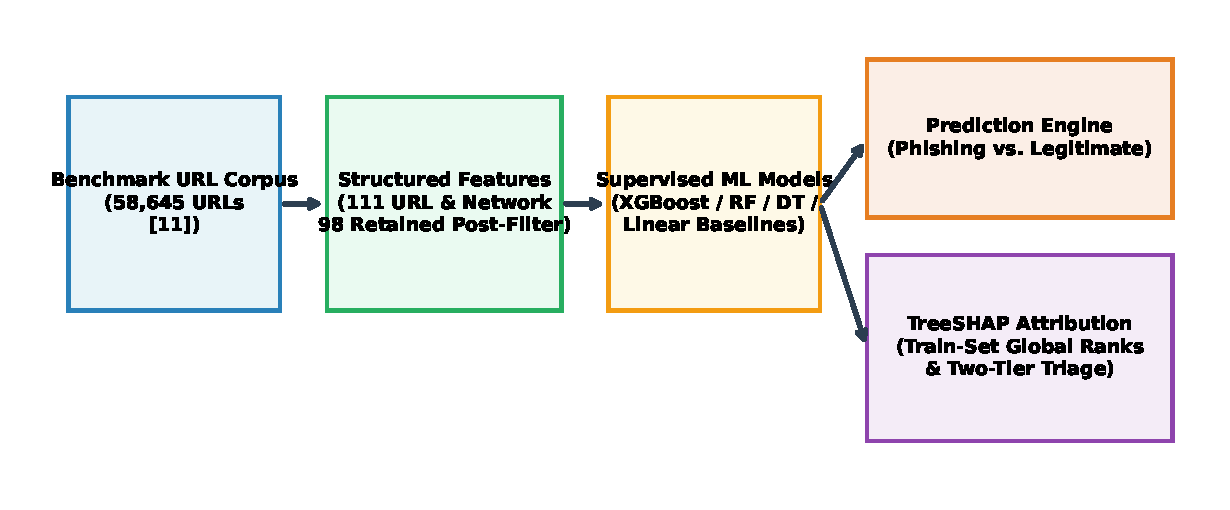
\includegraphics[width=0.88\columnwidth]{figures/fig1_system_architecture.pdf}
\caption{Architectural Pipeline of the Proposed Explainable Phishing Detection Framework.}
\label{fig:architecture}
\end{figure}

\subsection{Dataset Formulation and Preprocessing}
We utilize the benchmark dataset curated by Vrban{\v{c}}i{\v{c}} et al. \cite{vrbancic2020datasets}, containing 58,645 URLs (30,647 phishing from PhishTank/OpenPhish and 27,998 legitimate from Alexa top sites, search results, and open community directories). Table~\ref{tab:dataset} outlines the dataset parameters.

\begin{table}[htbp]
\caption{Dataset Specification and Partitioning}
\label{tab:dataset}
\centering
\resizebox{\columnwidth}{!}{
\begin{tabular}{lp{4.5cm}}
\hline
\textbf{Property} & \textbf{Specification / Value} \\
\hline
Dataset Provenance & Vrban\v{c}i\v{c} et al. (\textit{Data in Brief}, 2020) \cite{vrbancic2020datasets} \\
Feature Modality & Static URL Lexical, Path, File, Query, and Resolver \\
Total URL Instances & 58,645 URLs \\
Raw Feature Dimensions & 111 Numeric Features (97 Lexical / 14 Resolver; 96/15 in \cite{vrbancic2020datasets}) \\
Retained Dimensions & 98 Informative Features (13 Constant Domain Delimiters Filtered) \\
Target Class & Binary: Phishing (1) vs. Legitimate (0) \\
Phishing Instances & 30,647 (52.26\%) \\
Legitimate Instances & 27,998 (47.74\%) \\
Train / Test Partition & 80\% Stratified Train (46,916) / 20\% Test (11,729) \\
Missing / Sentinel Values & 0 NaN (Unset/unavailable metrics encoded as $-1$) \\
\hline
\end{tabular}
}
\end{table}


\begin{figure}[htbp]
\centering
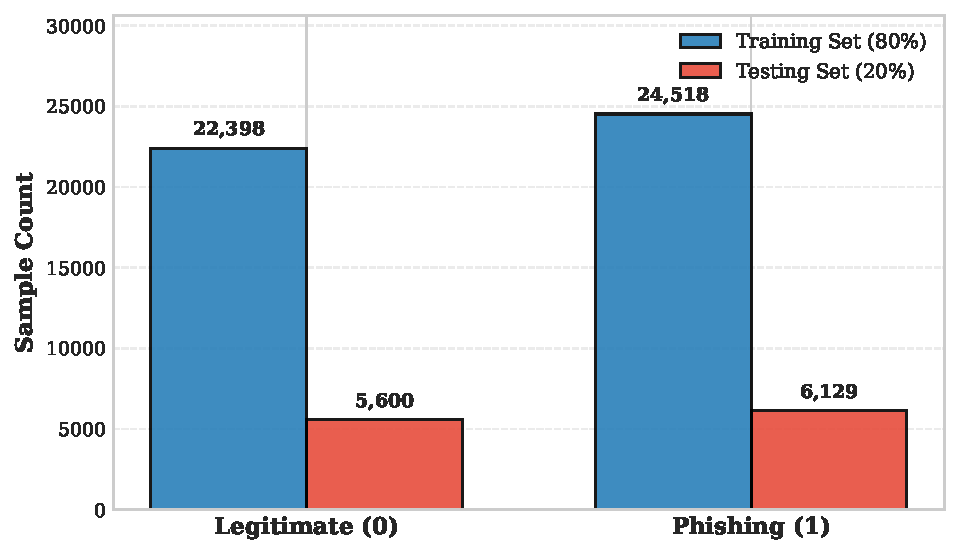
\includegraphics[width=0.88\columnwidth]{figures/fig2_class_distribution.pdf}
\caption{Class distribution across stratified train (80\%) and test (20\%) partitions.}
\label{fig:class_dist}
\end{figure}

As shown in Fig.~\ref{fig:class_dist}, the dataset is partitioned into an 80\% training corpus ($N_{\text{train}} = 46,916$) and a 20\% held-out test corpus ($N_{\text{test}} = 11,729$) using stratified sampling to preserve the 52.26\% : 47.74\% class distribution across partitions. Let $\mathcal{D} = \{(\mathbf{x}_i, y_i)\}_{i=1}^N$ denote the dataset, where $\mathbf{x}_i \in \mathbb{R}^D$ ($D=111$) and $y_i \in \{0, 1\}$. 

A cross-partition feature vector audit reveals that across the 98 retained features, exactly 335 test instances (2.86\% of the 11,729 test set) share identical feature vectors with instances in the training set. Within partitions, 906 rows in train (1.93\%) and 130 rows in test (1.11\%) represent internal duplicates. This occurs because distinct root-level URLs that lack path/query strings and share common registrar or default $-1$ values collapse to identical discrete feature vectors. Crucially, 332 of the 335 cross-partition twin pairs (99.1\%) share identical ground-truth labels (with only 3 label conflicts, 0.9\%). Evaluating on the strictly de-duplicated test subset ($N = 11,394$, where all 335 cross-partition twins are removed), XGBoost achieves 94.71\% accuracy and 95.05\% F1-score, while Random Forest achieves 94.18\% accuracy and 94.58\% F1-score (compared to 94.82\% / 95.05\% and 94.30\% / 94.57\% on the full test set), verifying that cross-partition repetition does not inflate generalization metrics.

A fundamental structural characteristic of this dataset is the use of the numeric sentinel $-1$ to denote ``not applicable'' or ``lookup unavailable'' (e.g., URLs lacking directory paths or query strings assign $-1$ to path/query metrics, and failed/unresolved WHOIS lookups assign $-1$ to activation age). This design preserves complete matrix density while encoding structural absence. Preprocessing fits a zero-variance filter $\mathcal{V}(X_j) = \frac{1}{N_{\text{train}}} \sum_{i=1}^{N_{\text{train}}} (x_{ij} - \mu_j)^2 > 0$ strictly on $\mathcal{D}_{\text{train}}$. Thirteen constant features (all belonging to the domain structural family) are eliminated, leaving $D' = 98$ informative features (84 lexical/structural and 14 network/resolver metrics). For distance-based models (Logistic Regression and Linear SVM), features are standardized via z-score scaling $z_{ij} = (x_{ij} - \mu_j)/\sigma_j$ fitted exclusively on $\mathcal{D}_{\text{train}}$.

\subsection{URL Feature Engineering Taxonomy}
The 111 structured metrics span six cybersecurity feature families ($20 + 21 + 18 + 18 + 20 + 14 = 111$ raw; $20 + 8 + 18 + 18 + 20 + 14 = 98$ retained). In the original benchmark specification \cite{vrbancic2020datasets}, the authors report 96 features extracted directly from URL strings and 15 extracted via custom Python logic (consisting of 14 external resolver metrics alongside \texttt{email\_in\_url}). In our framework, \texttt{email\_in\_url} is classified as an in-memory URL lexical metric because regex checking for an email pattern within a raw URL string requires zero external network queries or socket handshakes. Thus, we delineate 97 lexical/structural features (84 retained) and 14 external resolver features:
\begin{enumerate}
    \item \textbf{URL Lexical} (20/20 retained): URL character length (\texttt{length\_url}), presence flags (\texttt{email\_in\_url}), and delimiter frequencies (\texttt{qty\_slash\_url}, \texttt{qty\_dot\_url}, \texttt{qty\_hyphen\_url}, \texttt{qty\_equal\_url}, \texttt{qty\_and\_url}).
    \item \textbf{Domain Structural} (21/8 retained): Domain string length (\texttt{domain\_length}), IP indicator (\texttt{domain\_in\_ip}), authority dots (\texttt{qty\_dot\_domain}), vowels, and hyphens. Thirteen zero-variance domain delimiters (e.g., slashes, question marks, and symbols within domain authority) are eliminated.
    \item \textbf{Directory/Path} (18/18 retained): Directory character length (\texttt{directory\_length}), slash count (\texttt{qty\_slash\_directory}), and path delimiters (encoded as $-1$ when no directory is present).
    \item \textbf{File-Level} (18/18 retained): Filename length (\texttt{file\_length}) and character counts.
    \item \textbf{Query/Parameter} (20/20 retained): Query length (\texttt{params\_length}), parameter count (\texttt{qty\_params}), and argument delimiters.
    \item \textbf{Resolver/Network} (14/14 retained): Passive and active external lookups and search indicators: HTTP response latency (\texttt{time\_response}), SPF record flag (\texttt{domain\_spf}), Autonomous System Number (\texttt{asn\_ip}), domain activation age (\texttt{time\_domain\_activation}), domain expiration time (\texttt{time\_domain\_expiration}), resolved IP count (\texttt{qty\_ip\_resolved}), authoritative nameserver count (\texttt{qty\_nameservers}), MX mail server count (\texttt{qty\_mx\_servers}), DNS TTL (\texttt{ttl\_hostname}), TLS/SSL certificate status (\texttt{tls\_ssl\_certificate}), redirect hop count (\texttt{qty\_redirects}), URL Google index status (\texttt{url\_google\_index}), domain Google index status (\texttt{domain\_google\_index}), and URL shortener lookup flag (\texttt{url\_shortened}). Filtering 13 constant domain delimiters leaves exactly 84 purely in-memory lexical and structural features across groups 1--5 that require strictly 0 external network lookups.
\end{enumerate}

\subsection{Classification Model Architectures}
We evaluate five diverse classification paradigms: (i) \textbf{Logistic Regression (LR)} with L2 regularization ($C=1.0$); (ii) \textbf{Decision Trees (DT)} with Gini impurity splitting ($\text{max\_depth}=12$); (iii) \textbf{Random Forest (RF)} ensemble with 100 bagging trees ($\text{max\_depth}=15$); (iv) \textbf{Linear SVM} with Platt calibration; and (v) \textbf{XGBoost} \cite{chen2016xgboost} (100 estimators, $\text{max\_depth}=6$, $\eta=0.1$, subsample=0.8, colsample=0.8), minimizing the regularized objective: $\mathcal{L}^{(t)} = \sum_{i=1}^N l\left(y_i, \hat{y}_i^{(t-1)} + f_t(\mathbf{x}_i)\right) + \gamma T + \frac{1}{2}\lambda \sum_{j=1}^T w_j^2$. Table~\ref{tab:model_config} lists the detailed hyperparameters.

\begin{table}[htbp]
\caption{Model Hyperparameter Configurations}
\label{tab:model_config}
\centering
\resizebox{\columnwidth}{!}{
\begin{tabular}{lp{4.5cm}}
\hline
\textbf{Model Architecture} & \textbf{Hyperparameter Specification} \\
\hline
Logistic Regression & L2 penalty, $C=1.0$, L-BFGS solver, max\_iter=1000 \\
Decision Tree & Gini impurity, max\_depth=12, min\_samples\_split=10 \\
Random Forest & 100 trees, max\_depth=15, min\_samples\_split=5 \\
Linear SVM & LinearSVC ($C=1.0$), Platt calibrated (3-fold CV) \\
XGBoost & 100 estimators, max\_depth=6, $\eta=0.1$, subsample=0.8, colsample=0.8, histogram method \\
\hline
\end{tabular}
}
\end{table}


\subsection{Explainable AI via TreeSHAP}
To explain model decisions, we deploy TreeSHAP \cite{lundberg2020local, lundberg2017unified}, which satisfies the additive attribution property $f(\mathbf{x}) = \phi_0 + \sum_{j=1}^{D'} \phi_j(\mathbf{x})$, where $\phi_0 = \mathbb{E}[f(\mathbf{x})]$ is the expected base model output, and $\phi_j(\mathbf{x})$ is the Shapley attribution:
\begin{equation}
\phi_j(\mathbf{x}) = \sum_{\mathcal{S} \subseteq \mathcal{F} \setminus \{j\}} \frac{|\mathcal{S}|! (|\mathcal{F}| - |\mathcal{S}| - 1)!}{|\mathcal{F}|!} \left[ f(\mathcal{S} \cup \{j\}) - f(\mathcal{S}) \right]
\label{eq:shap_formula}
\end{equation}

Global feature importance $I_j$ is computed as the mean absolute SHAP value strictly over a training explanation subset $\mathcal{X}_{\text{train, exp}} \subset \mathcal{D}_{\text{train}}$ ($N=500$ random samples): $I_j = \frac{1}{|\mathcal{X}_{\text{train, exp}}|} \sum_{i \in \mathcal{X}_{\text{train, exp}}} |\phi_j(\mathbf{x}_i)|$. Deriving $I_j$ exclusively on $\mathcal{D}_{\text{train}}$ establishes train-only attribution and prevents selection leakage into feature selection. Under model retraining across independent seeds (varying tree subsampling), global feature rankings demonstrate high stability: $\rho_s = 0.973 \pm 0.010$ Spearman rank correlation across all 98 features, Kendall's $\tau = 0.7948 \pm 0.031 \approx 0.79$ within the top-20 features, and 95.0\% top-20 set overlap (19 of 20 features preserved across all retrained models). When fixing the model and varying only the explanation subsampling seed, rankings show near-perfect agreement ($\rho_s = 0.9991$, Pearson $r = 0.9995$, Kendall's $\tau = 0.9131$ within top-20, 100\% top-20 set overlap; $\rho_s = 0.9995$ between $N=500$ and $N=1,000$), confirming that high stability is robust and not an artifact of tied near-zero features in the tail. Ranked features $I_{(1)} \ge I_{(2)} \ge \dots \ge I_{(D')}$ direct nested feature pruning.

